\chapter{Background}
\label{chapter:background}
This chapter will provide the essential background needed to understand the technical chapters of this thesis. It will study any necessary terminology and techniques used throughout the thesis, covering knowledge about finances, flattening and CUDA.

\section{Financial background}
Derivatives have become important in finance in the last 30 years with futures and options actively traded worldwide. The derivatives market is much bigger than the stock market when underlying assets are measured. Derivatives can be used for hedging, speculation or arbitrage as they transfer a wide range of risks in the economy from one entity to another. A \textit{derivative} is a financial instrument with a value that derives from the value of some other basic underlying asset.~\cite[pg.1]{ofod}

\subsection{Options}
This thesis will focus on only one specific type of derivatives - \textit{options}. These are contracts that give the holder the right to buy or sell an underlying asset at a certain point in time for a certain price, both specified when purchasing the option. This is in contrast with other derivatives - \textit{forwards} and \textit{futures}, where the holder is obligated to buy or sell the underlying asset. 

\paragraph{}
There are two types of options. A \textit{call option} gives the holder the right to buy the underlying asset by a certain date for a certain price. A \textit{put option} gives the holder the right to sell the underlying asset by a certain date for a certain price. The price in the contract is called \textit{strike price} and the expiration date is called \textit{maturity}. Options that can be exercised at any time before maturity are known as \textit{American options} and options that can be exercised only on the expiration date itself are known as \textit{European options}. One contract usually allows to buy or sell 100 shares.~\cite[pg.7-8]{ofod}
\paragraph{Example}
An investor spent 20.000 kr for an option to buy 100 Maersk shares for 9.600 kr each. The current market price for Maersk stock is 9.440 kr as of March 15, 2018. If the price does not rise above 9.600 kr by the maturity, the investor does not exercise the option and loses 20.000 kr. However, if Maersk stock is priced at 10.000 kr when the option can be exercised, the investor is able to buy 100 shares for the strike price of 9.600 kr and immediately sell them for 10.000 kr. This will generate a profit of $400 * 100 = 40.000$ kr minus the initial contract cost of 20.000 kr.

Table~\ref{table:option-sell} illustrates an example of exercising this option at different dates. Even if the stock price rises above the strike price, the net profit might still be negative when the contract price is accounted for.  

\begin{table}[h]
\centering
\caption{Profit generated by a call option with strike price of 9.600 kr and contract price of $100 \times 200 = 20.000$ kr.}
\label{table:option-sell}
\begin{tabular}{|l|l|l|l|l|}
\hline
                       & March 2018    & June 2018 & Sept. 2018 & Dec. 2018 \\ \hline
Stock price (kr)       & 9.440         & 9.700     & 10.000         & 9.800         \\ \hline
Share sale profit (kr) & not exercised & 10.000    & 40.000         & 20.000        \\ \hline
Net profit (kr)        & -20.000       & -10.000   & 20.000         & 0             \\ \hline
\end{tabular}
\end{table}

\subsection{Bonds}
Bonds are a form of debt that allow companies or governments borrow money from investors. Most bonds periodically paid coupons (interest) to the holder. The principal payment (known as face value or par value) is paid at the end of bond's life.~\cite[pg.80]{ofod}

\paragraph{Zero rates}
Interest rate on an investment that starts today and lasts for $n$ years are called $n$-year zero-coupon interest rates. All the interest and principal is realized at the end. For example, an investment of 100\$ with a 5-year zero rate with continuous compounding at 5\% p.a. grows to~\cite[pg.80]{ofod}
\begin{equation*}
    100 \times e^{0.05 \times 5} = 128.40
\end{equation*}

% \subsection{Mean reversion}
%  An important property of interest rates is that they appear to be pulled back to some long-run average level over time. This phenomenon is known as mean reversion. When the short rate is high, mean reversion tends to cause it to have a negative drift; when the short rate is low, mean reversion tends to cause it to have a positive drift. Mean reversion is illustrated in fig. \ref{fig:meanreversion}\cite{ofod}.

\paragraph{Bond pricing}
The theoretical price of a bond can be calculated as the present value of all cash flows received by the holder. For example, there is a 2-year bond with 100\$ principal that pays coupons at the rate of 6\% semiannually. When the zero rates are as in table~\ref{table:zero-rates}, we can calculate the present value of the first coupon of 3\$ by discounting it at 5.0\% for 6 months, second coupon at 1 year and so on. Then the theoretical price of the bond is~\cite[pg.80-81]{ofod}
\begin{equation*}
    3e^{-0.05 \times 0.5} + 3e^{-0.058 \times 1.0} + 3e^{-0.064 \times 1.5} + 103e^{-0.068 \times 2.0} = 98.39
\end{equation*}

\begin{table}[h]
\centering
\caption{Zero rates used for bond pricing}
\label{table:zero-rates}
\begin{tabular}{|l|l|}
\hline
Maturity (years) & \begin{tabular}[c]{@{}l@{}}Zero rate (\%)\\ (continuously compounded)\end{tabular} \\ \hline
0.5              & 5.0                                                                                \\ \hline
1.0              & 5.8                                                                                \\ \hline
1.5              & 6.4                                                                                \\ \hline
2.0              & 6.8                                                                                \\ \hline
\end{tabular}
\end{table}

\paragraph{Bond yield}
A bond's yield is the single discount rate that gives a bond price equal to its market price. Continuing the pricing example, the yield $y$ can be computed as
\begin{equation*}
    3e^{-y \times 0.5} + 3e^{-y \times 1.0} + 3e^{-y \times 1.5} + 103e^{-y \times 2.0} = 98.39
\end{equation*}
This equation gets solved by setting $y = 6.76\%$.~\cite[pg.81]{ofod}

\subsection{Volatility}
Volatility is a statistical measure showing the uncertainty of the returns of a given security or a market index \cite{ofod}[pg. 303]. The higher the volatility, the higher the risk of the security will be. In the one-factor Hull–White model, mean reversion causes the forward rate volatility to be a declining function of the maturity\cite{ofod}[pg. 698]. 
% 30.5 in HW, 14.4 in example of stocks 

\subsection{Day-count conventions}
Day-count conventions is a method for computing the amount of accrued\footnote{accumulated or received payments or benefits over time.} interest or the present value when the next coupon payment is less than a full coupon period away. Typically, bond markets and financial instruments have their own day-count conventions, which vary on the type of instrument, the interest rate type, and the issuance country. 
% 28.8 https://en.wikipedia.org/wiki/Day_count_convention

\subsection{Trinomial trees}
Determining the value of a derivative is key to successful/profitable options trading. There are various ways of pricing options and some of the more common ones are the Black-Scholes model\cite{blackscholes}, binomial and trinomial trees. Using the Black-Scholes formula, requires several assumptions to be made: 
\begin{itemize}
    \item The option must be European and can only be exercised at expiration.
    \item No dividends are paid out during the life of the option.
    \item Markets are efficient (i.e., market movements cannot be predicted).
    \item There are no transaction costs in buying the option.
    \item The risk-free rate and volatility of the underlying are known and constant.
    \item The returns on the underlying are normally distributed.
\end{itemize}
Constructing binomial trees on the other hand is a far more flexible approach. It valuations for a derivative to be performed on each node in a span of time (analytical tractability), as well as can be used on other, path-dependent derivatives, such as exotic options. 

Furthermore, the trinomial option pricing model is quite similar to binomial trees, with the difference that it consolidates another possible value per one time period. This makes the trinomial model even more relevant to real life situations, as it ensures the possibility that the value of the underlying asset may not change over a time period. Last, but not least, tree methods are much simpler to use than the Black-Scholes model, as they are dependent only on a few stochastic variables at most.

\subsection{Mean reversion}
One-factor short-rate models are one such example, where the tree is dependent on a single stochastic factor – the short rate\footnote{A mathematical model that describes the future evolution of interest rates.}. In short-rate models, on the long run, interest rates appear to be drawn back to their average level over time\cite{ofod}[pg. 684]. This phenomenon is known as \textbf{mean reversion}. When the short rate - typically denoted as r - is high, mean reversion tends to cause the interest rates to decrease; vice verse, when r is low, mean reversion tends to cause them to increase. This is explained visually on fig. \ref{fig:background:meanreversion} below. 

\begin{figure}[H]
	\centering
	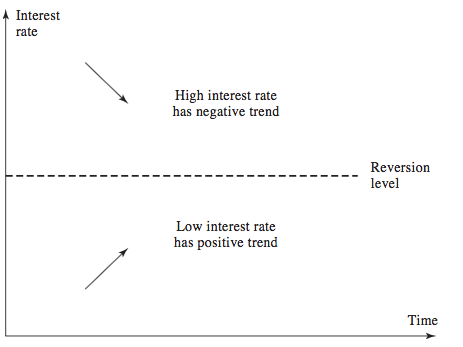
\includegraphics[width=0.8\textwidth]{img/meanreversion.png}
	\caption{Illustration of mean reversion}
	\label{fig:background:meanreversion}
	\source{Based on Options, Futures and Other Derivatives\cite{ofod}[pg. 684].}
\end{figure}

Unlike other methods, trinomial trees conveniently incorporate mean-reversion, by using a width limit and modified branching methods for the tree. Standard branching(see fig.\ref{fig:background:standardbranching}) remains the same throughout the tree. At the bottom of the tree, where interest rates are very low, the ‘‘up one/straight along/down one’’(see fig.\ref{fig:background:altbranchingbottom}) branching is used. At the top of the tree, where interest rates are very high, the ‘‘straight along/down one/ down two’’ branching is used (see fig.\ref{fig:background:altbranchingtop}). 

\begin{figure}[H]
\centering
\begin{subfigure}{.3\textwidth}
  \centering
  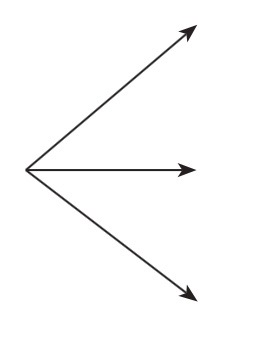
\includegraphics[width=.7\linewidth]{img/standardbranch.jpg}
  \caption{Standard branching}
  \label{fig:background:standardbranching}
\end{subfigure}
\begin{subfigure}{.3\textwidth}
  \centering
  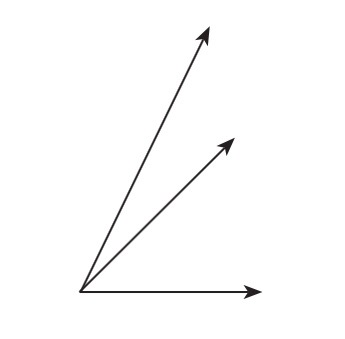
\includegraphics[width=.93\linewidth]{img/bottombranch.jpg}
  \caption{Bottom branching}
  \label{fig:background:altbranchingbottom}
\end{subfigure}
\begin{subfigure}{.3\textwidth}
  \centering
  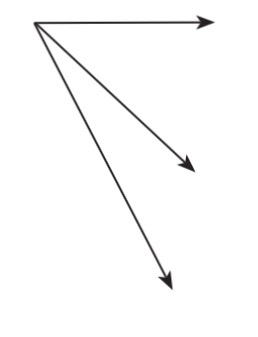
\includegraphics[width=.7\linewidth]{img/topbranch.jpg}
  \caption{Top branching}
  \label{fig:background:altbranchingtop}
\end{subfigure}
\caption{Alternative branching methods for a trinomial tree.}
\label{fig:background:allbranchings}
\source{Based on Options, Futures and Other Derivatives\cite{ofod}[pg. 698].}
\end{figure}

\subsection{Yield curve}
Typically for most pricing models, the probability distributions of interest rates, bond prices, or other variables at a future point in time are lognormal. However, this does not provide any information of how interest rates evolve over time. \cite{ofod}[pg. 682]. This can achieved by building a term structure model, also known as a yield curve. The term structure model describes the evolution of all zero-coupon interest rates. For simplicity, in this thesis we have chosen to use the yield curves provided by the book examples.
% a.k.a. term structure section 30.1 and intro to chapter 30

\subsection{Other numerical methods}
Beside the Black-Scholes method and the binomial/trinomial tree approaches, there are yet other popular means for valuing derivatives. They have their advantages, but are either much more inefficient in terms of computation time, or perform similarly to trinomial trees. 

\textbf{Monte Carlo} simulations is a method, where different paths are sampled to obtain the expected payoff of the asset in a risk-neutral world and are then discounted at this risk-free rate. The key advantage of Monte Carlo simulations is their ability to be used when the payoff depends on the path followed by the underlying single-market variable, as well as when it depends only on the final value of this variable. Unfortunately, the method consumes a high computation time and cannot easily handle situations with early exercise opportunities \cite{ofod}[pg. 448].   
% 20.6
% - Monte Carlo simulations

% 20.8
\textbf{Finite difference methods (FDM)} value a derivative by solving the differential equation that the derivative satisfies. The differential equations are converted into sets of difference equations and are are solved iteratively. This is similar to the trinomial trees method, since the computations also work back from the end of the derivative maturity to the beginning. The explicit finite difference method is functionally the same as using a trinomial tree, while the implicit finite difference method takes far longer computational time\cite{ofod}[pg.455 - 466].

%%%% FLATTENING BACKGROUND %%%%
\section{Flattening background}
As briefly mentioned in the Introduction, complex applications are often composed of multiple nested levels of operations. These include i.e. for-loops, if-then-else statements, etc. In order to effectively utilize massively parallel hardware, it is necessary that nested higher-order functions are properly flattened, which can be done with the use of certain flattening techniques such as the ones described in this section. Note that only flattening transformations that have been used in this project are described, even though many other transformations can be composed.  

\subsection{Nested map in a map}
\label{chapter:section:flattening:map}
The $\mathit{map}$ function applies a given function to each element of a list. A nested map inside a map is one of the simplest flattening transformations that can be performed. The procedure is as simple as applying the nested map on the flattened array. E.g. suppose we have a nested function $\mathit{f(x)=x+1}$, applied on each of the nested elements of the array $\mathit{x=[[1,2,3],[4,5,6]]}$. This is done separately on both of the nested arrays, resulting in $\mathit{[[2,3,4],[5,6,7]]}$. The same operation would result in $\mathit{[2,3,4,5,6,7]}$, when the array is flat. This is also the expected outcome. 

\subsection{Nested scan in a map}
\label{chapter:section:flattening:scan}
The $\mathit{scan}$ function takes as input a combining operator, a neutral element and an array. The operator is used consequently on all elements of the array, either by starting with the neutral, or with the first element in the array. These two different ways are called exclusive and inclusive scan respectively. This is very similar to $\mathit{reduce}$ with the difference that using $\mathit{scan}$ allows intermediate results to be kept in the returned result. E.g. suppose an array $\mathit{x=[[2, 3, 4],[5, 6, 7]]}$ is given and scan is performed with the $\mathit{(+)}$ operator and a neutral element $\mathit{0}$. An inclusive scan returns $\mathit{[[2, 5, 9], [5, 11, 18]]}$ for each of the nested arrays, while an exclusive scan similarly returns \\ $\mathit{[[0, 2, 5],[0, 5, 11]]}$, as it starts from the neutral element. On a flat array, scan is replaced by a segmented scan, which also takes a flag array as an input argument. The flag array indicates the positions and lengths of the nested arrays. E.g. the flag array will be $\mathit{[3,0,0,3,0,0]}$ on the example above and the complete transformation:\\ $\mathit{sgmScanInc}\:\mathit{(+)}\:\mathit{0}\:\mathit{[3,0,0,3,0,0]}\:\mathit{[2,3,4,5,6,7]}\:\equiv\:\mathit{[2,5,9,5,11,18]}$ and\\ $\mathit{sgmScanExc}\:\mathit{(+)}\:\mathit{0}\:\mathit{[3,0,0,3,0,0]}\:\mathit{[2,3,4,5,6,7]}\:\equiv\:\mathit{[0,2,5,0,5,11]}$.

\subsection{Nested replicate in a map}
\label{chapter:section:flattening:replicate}
The \textit{replicate} function is used to create an array of \textit{n} exact copies of a number. The example shown below assumes 3 elements - \textit{ms=[0.0, 1.0, 2.0]} - replicated \textit{ns=[3,5,7]} times respectively. The flattening of a replicate nested inside a map is achieved by the following steps:
\begin{itemize}
    \item Compute an array of indexes - \textit{inds} - by using additive exclusive scan on \textit{ns}. In the example above, the result of this step should be \textit{inds=[0, 3, 8]}
    
    \item Compute the size - \textit{s} - of the target array. This can be done in multiple ways, one of which is by summing the last elements of \textit{inds} and the last element of \textit{ns}. This is \textit{s=8+7=15} in the given example.
    
    \item Compute a \textit{flags} array, by writing \textit{ns} into an array of size \textit{s} with zeros, at the locations indicated by the $\mathit{inds}$ array. In the given example, the results would be \textit{flags=[3, 0, 0, 5, 0, 0, 0, 0, 7, 0, 0, 0, 0, 0, 0]}. 
    
    \item Compute a \textit{vals} array, by writing the values to be replicated - \textit{ms} - into an array of size \textit{s} with zeros, at the locations indicated by the $\mathit{inds}$ array. In the given example, the results would be \textit{flags=[0.0, 0.0, 0.0, 1.0, 0.0, 0.0, 0.0, 0.0, 2.0, 0.0, 0.0, 0.0, 0.0, 0.0, 0.0]}. 
    
    \item Compute the flattened nested replicate by performing an inclusive segmented scan on \textit{flags} with \textit{vals}. This results in \textit{result=[0.0, 0.0, 0.0, 1.0, 1.0, 1.0, 1.0, 1.0, 2.0, 2.0, 2.0, 2.0, 2.0, 2.0, 2.0]}.
\end{itemize}
\newpage
\subsection{Nested reduce in a map}
\label{chapter:section:flattening:reduce}
A $\mathit{reduce}$ is another higher-order function which uses a given combining operator and a neutral element. It recursively processes its elements with the operator, building up a return value.
As previously mentioned, this is quite similar to an inclusive scan operation, with the only difference that $\mathit{reduce}$ does not keep intermediate values. I.e. consider the nested array $\mathit{x=[[1,3,4],[6,7]]}$. A $\mathit{reduce}$ with a $\mathit{(+)}$ operator will produce $\mathit{8}$ and $\mathit{13}$ for the respective nested arrays. A flattened reduce should accordingly result in the array $\mathit{[8, 13]}$. A flattened reduce takes one more input argument - $\mathit{flags}$ - and comprises of a scan-pack composition, with the following steps:
\begin{itemize}
    \item Perform an additive inclusive segmented scan with $\mathit{flags=[1, 0, 0, 1, 0]}$ and $\mathit{x=[1, 3, 4, 6, 7]}$ in the example above. The result of this step will then be  $\mathit{vals=[1, 4, 8, 6, 13]}$. 
    
    \item Shift $\mathit{flags}$ left by 1, by applying the map $\mathit{if}\;\mathit{i}\;\mathit{<}\;\mathit{n-1}\;\mathit{then}\;\mathit{flags[i+1]}\;\mathit{else}\;\mathit{1}$ over the iterator from $\mathit{0}$ to the length of $\mathit{x}$. In the example above, this becomes $\mathit{sgm\_end=[0,0,1,0,1]}$.
    
    \item Compute $\mathit{inds0}$ by using an inclusive scan on the flags. $\mathit{inds0=[1,1,1,2,2]}$
    
    \item Obtain $\mathit{inds}$ by applying the map\\ $(i,e)\;->\;\mathit{if}\;\mathit{e}\;\mathit{>}\;\mathit{0}\;\mathit{then}\:\mathit{i-1}\;\mathit{else}\;\mathit{-1}$ on $\mathit{inds0}$ and $\mathit{sgm_end}$. This becomes $\mathit{inds=[-1,-1,0,-1,1]}$.
    
    \item Compute the end result by writing $\mathit{vals}$ on the $\mathit{inds}$ indexes to an empty array of size the last element of $\mathit{inds0}$, i.e., $\mathit{res=[8,13]}$
\end{itemize}

%%%%% CUDA Background %%%%%
\section{CUDA background}
\subsection{Roadmap}
Short about: Kernels, Grids, Blocks, Threads, Warps, GPU Compute capability, Device <-> Host, something more ? 
\subsection{Process flow}
% https://en.wikipedia.org/wiki/CUDA
\subsection{Memory coalescing}

\section*{Summary}
This chapter has provided a brief introduction to to the necessary knowledge needed to understand the following chapters. This has covered financial topics such as options, volatility, trinomial trees, and more, all needed in the implementations. Following was the flattening background needed for applying transformations in order to exploit thread divergence and experiment with different levels of nested parallelism. Finally, we have introduced the basics needed to understand terminology and techniques in CUDA, which have been all throughout this thesis. The following chapter will study the Hull-White Single-Factor Model, in order to explore its mechanisms and prepare an implementation strategy.